\documentclass[a4paper, 12pt]{article}

\usepackage{babel}
\usepackage{enumitem}
\usepackage{times}
\usepackage{graphicx}
\usepackage{geometry}
	\geometry{left = 4cm, top = 4cm, right = 3cm, bottom = 3cm}
\usepackage{float}
\usepackage{setspace}
	\setstretch{1.5}
\usepackage{listings}


\begin{document}
\title{\textbf{Tugas Modul Praktikum Pemrograman II}}
\date{}

\maketitle

\begin{figure}[!ht]
\begin{center}

\includegraphics[width = 4cm, height = 3.5cm]{gambar/logo.png}
\end{center}
\end{figure}

\begin{center}
\vspace{1cm}
Disusun Oleh:\\
Faris Muhammad Ihsan\\
D4 TI 2B\\
1.18.4.099\\
\vspace{1cm}
\textbf{PROGRAM DIPLOMA IV POLITEKNIK POS INDONESIA} \linebreak
\textbf{POLITEKNIK POS INDONESIA} \linebreak
\textbf{BANDUNG}\linebreak
\textbf{2019}

\end{center}

\thispagestyle{empty}

\begin{center}
\title{\LARGE\bf Chapter 2}\\
\title{\LARGE \bf Pemrograman Dasar}\\
\end{center}

\appendix
\section{Teori}

\begin{enumerate}
\item Variable\\ 
Variable adalah tempat penyimpanan sementara untuk data yang dapat berupa integer, string, boolean, float, dan array. cara menggunakan variable pada python hampir sama dengan bahasa lainnya hanya perlu menuliskan "nama\textunderscore Variabel = data". Penggunaan variabel tidak boleh menggunakan keyword yang sudah ada, tidak boleh diawali dengan \textunderscore dan variabel bersifat case sensitive.

\item Input dan Output\\
Untuk memberikan inputan oleh user diperlukan kode "inputan = input(" ")"\\
Sedangkan untuk output ke user menggunakan "print("inputan")"

\item OperatorAritmatika\\
\begin{tabular}{|c|c|}
\hline
Operator & Simbol\\
\hline
Penjumlahan & +\\
\hline
Pengurangan & -\\
\hline
Perkalian & *\\
\hline
Pembagian & /\\
\hline
Modulus & \% \\
\hline
Pemangkatan & **\\ 
\hline
\end{tabular}

Untuk mengubah string ke integer type data string harus dilakukan casting dengan cara "int(variable)". Sedangkan untuk integer ke string menggunakan "str(variable)".

\item Syntax Perulangan
\begin{enumerate}[label=\alph*.]
\item for\\
Contoh:\\ 
ulang = 10
for i in range(ulang):\\
print "ulang ke"+str(i)
\item while
While digunakan untuk perulangan yang tidak pasti. Contoh:\\
i=0\\
while True:\\
	if i < 0\\
		print("Saat ini i bernilai: "), i\\
		i = i + 1\\
	elif i >= 10:\\
		break\\

\item Kondisi\\
Contoh If:
\lstinputlisting[language=Python]{src/if.py}

if bersarang\\
\lstinputlisting[language=Python]{src/ifnested.py}

\item Error\\
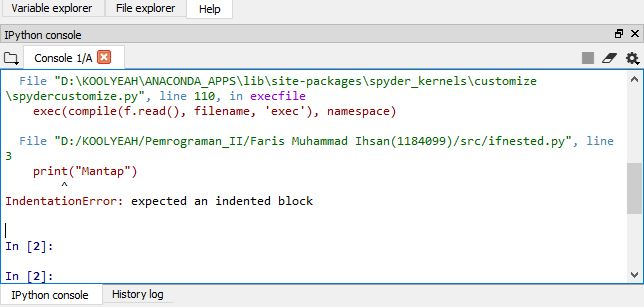
\includegraphics{gambar/errsyntax.jpg}
cara mengatasinya hanya memberikan identasi saja

\item Cara memakai try except\\
\lstinputlisting[language=Python]{src/except.py}

\end{enumerate}

\section{Keterampilan Perograman}

\begin{enumerate}

\item
\lstinputlisting[language=Python]{src/NPM1.py}

\item
\lstinputlisting[language=Python]{src/NPM2.py}

\item
\lstinputlisting[language=Python]{src/NPM3.py}

\item
\lstinputlisting[language=Python]{src/NPM4.py}

\item
\lstinputlisting[language=Python]{src/NPM5.py}

\item
\lstinputlisting[language=Python]{src/NPM6.py}

\item
\lstinputlisting[language=Python]{src/NPM7.py}

\item
\lstinputlisting[language=Python]{src/NPM8.py}

\item
\lstinputlisting[language=Python]{src/NPM9.py}

\item
\lstinputlisting[language=Python]{src/NPM10.py}

\item
\lstinputlisting[language=Python]{src/NPM11.py}

\end{enumerate}

\section{Keterampilan Penanganan Error}
\begin{enumerate}

\item Error\\
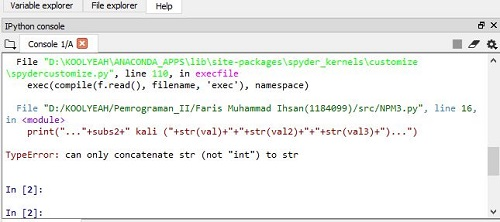
\includegraphics{gambar/2errpy.jpg}
Solusi yang dilakukan adalah mengcasting type data int menjadi str.

\item Penggunaan Try Except\\
\lstinputlisting[language=Python]{src/2err.py}

\end{enumerate}
\end{enumerate}
\end{document}

